\documentclass[a4paper,12pt]{article}
\usepackage{amsfonts}
\usepackage{amsmath}
\usepackage{amssymb}
\usepackage{graphicx}
\usepackage{natbib}
\usepackage{url}
\usepackage{geometry}%
\usepackage{algorithm}
\usepackage[noend]{algpseudocode}
\makeatletter
\def\BState{\State\hskip-\ALG@thistlm}
\makeatother


\pagenumbering{arabic}
\setcounter{page}{0}

%%%%% Define the title page
\title{SF2568: Project Report \\ Michael Hanke (\textit{hanke@nada.kth.se})}

\author{\hspace*{-0.5cm}
  \begin{tabular}{cc}
  Omar Elshenawy (\textit{omares@kth.se})\\ Thomai Stathopoulou (\textit{thomai@kth.se}) \\ 
  \end{tabular}
}
\date{}


%\pagestyle{fancy}
\setlength{\headheight}{15pt}
%\fancyhf{}



\begin{document}
	\maketitle
	

\thispagestyle{empty}	% To remove page number on title page


% Put in date at the end of title page
\vfill
\begin{center}
	\today
\end{center}
\clearpage		% Create new page	
	
	
\section{Problem Definition}
With the digitization of many medical devices, the images generated have grown higher in resolution and larger in quantity. MRI machines, produce a sequence that contains several hundred high resolution images, each image representing a slice of the tissue being filmed. Processing such sequences requires extensive computation. Doing such computations on one processor takes very long time. One of the most common processing procedures is to cluster the sequence of images in 3D, that is, connect different clusters that exist in each slice, with ones that exist in the next slice, which would correspond to segmenting a muscle or a bone. In the current project, a multi-core architecture is explored.
		
	\section{Proposed Algorithm}\label{sec:alg}
A common approach to solving the problem of detecting 3D clusters is to divide the problem into two parts, generate clusters on each image separately, then connect these clusters across images. This solution is map-reduce compatible. Therefore the problem is divided into two subtasks::
		\begin{enumerate}
			\item Segment each slice (Map) \label{task:1}
			\item Merge clusters of consecutive slices (Reduce) \label{task:2}
		\end{enumerate}
		\subsection{Segment each slice}
The first step is to segment each slice. Therefore the slices are distributed in a load-balanced linear data distribution manner. Basically, every processor gets a number of image slices $I_p$ which is calculated as follows:
			
			\begin{equation}
			I_p = \lfloor{\frac{N + P - p - 1}{P}}\rfloor,
			\end{equation}
			
where $N$ denotes the number of slices, $P$ the total number of processors used and $p$ the current active processor.

Each core computes a sequential k-means on its designated slices. This can be seen in details in Procedure \textit{Cluster} in Algorithm~\ref{algo}.
\subsection{Merge clusters of consecutive images}
The clusters that were generated in the previous step are then combined together into one set of clusters. This has to be done sequentially in order to maintain stability in the labels. This sequential merging was achieved by having each processor merge the labels of its preceding processor, and send its new set of labels to the following processor. This can be seen in details in Procedure \textit{Merge} in Algorithm~\ref{algo}.
		\begin{algorithm}
			\caption{3D K-means}\label{algo}
			\begin{algorithmic}[1]
				\Procedure{Cluster}{}
				\State $N \gets$ number of Slices
				\State $P \gets$ number of Processors
				\State $p \gets$ processor Id
				\State $\textit{p\_images} \gets $images[range($I_{p - 1}, I_{p - 1}+I_p - 1)$]$ $
				\For{$i$ in 0, length($p\_images$)}
				\State $labels[i] \gets$ k\_means(\textit{p\_images}[i])
				\State $blobs[i] \gets$ connected\_components($p\_images[i], labels[i]$)
				\EndFor
			
				\EndProcedure
				
				\Procedure{Merge}{}
				\State $c\_blobs \gets$ combine\_blobs($blobs[0], blobs$)
				\If {$p~!=0$}
					\State receive($previous\_blobs$)
					\State combine\_blobs($blobs, previous\_blobs$)\\
				\EndIf
					\State send($p+1, c\_blobs$)
				\EndProcedure
				\Procedure{combine\_blobs}{blobs, blobs\_list}
				\State $intersections \gets$ intersect\_blobs\_rectangle($blobs, blobs\_list$)
				\For{$i$ in 0, length($intersections$)}
					\State $new\_blobs \gets blobs[intersections[i]]$
				\EndFor
				\EndProcedure
			\end{algorithmic}
		\end{algorithm}
		
		
\section{Theoretical Performance Analysis}
Since our approach to the problem was that of an embarassingly parallel problem, we define the time complexity in terms of number of images processed per unit time. For Task~\ref{task:1}, the complexity of the algorithm for the sequential version is $O(N)$. Then, the complexity is $O(N/P)$ for the parallel version. For Task~\ref{task:2}, the complexity of the algorithm is again $O(N)$, and for the parallel version, it is the same.
	
	
\section{Implementation Details}
In order to be able to run the implemented code and check its performance, we needed to find a dataset containing MRI scans, in quantities and sizes that were large enough, so as to render the parallelization meaningful. However, since finding medical data is not easy, we decided to use a regular image.

We used a single image in two different sizes and replicated it in order to simulate the different slices of an MRI scan, where the number of slices was given as an input to the program.

When running the code locally, we are able to show the segmented slices, where the blobs are indicated by a numbered rectangle, where the number gives the label of the blob. After the merging of the clusters has occurred, the blobs of the different slices that correspond to a larger 3D segmentation have the same label.

When running the program on PDC, since it is not possible to show the images, we save the important information to a file, where each line gives us the slice number, blob label, coordinates and dimensions of the rectangle surrounding the blob.

\section{Example}
\begin{figure}
  \centering
  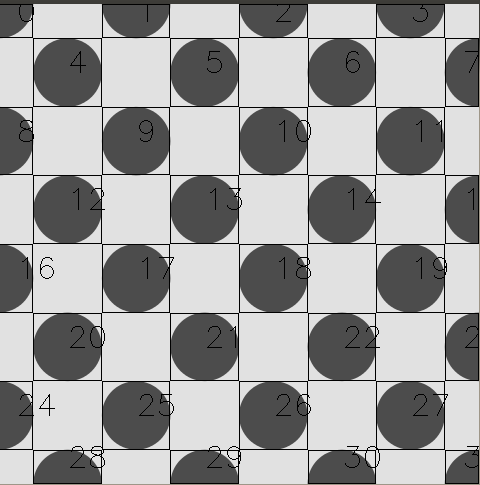
\includegraphics[scale=0.5]{example.png}
  \caption{Example of segmentation and blob labelling}
  \label{example}
\end{figure}

As an example in Figure~\ref{example} we can see that the different dots are detected and labelled correspondingly. A total number of 32 blobs has been detected. In the case of different slices (here we only see one), the adjacent blobs would be labelled accordingly. For example, the dot that lies ``under'' blob 21, would also be labelled as 21 so that we can know that it is one 3D blob.

\section{Experimental Speedup}
In order to be able to evaluate the performance of our implementation, we ran a number of experiments on multiple core with varying code parameters, such as the number of processors used, the size of the image and the number of slices.

In Figures~\ref{l_one_n} to~\ref{s_one_n_speed} we have collected most results of our experiments in compact graphs. The graphs show the run times and speed-ups in relation to the number of processors using increasing numbers of slices for an image sized $[1024 \times 1024]$ and $[768 \times 768]$.

First, we can notice in the graphs, that the different lines start and end on different points. That is, because depending on the size of the image, each processor has a limit of the number of slices it can handle memory-wise.

There is an obvious decrease in the run times with increasing number of processors. However, we can notice that for a constant work load the run times tend to stabilize after a certain addition of processors. That is an indication of Amdahl's law, showing that there is a certain speed-up that can be achieved for a fixed workload.

We can focus on the lines representing number of slices ranging in $[64 \ldots 256]$, which we assume to be a more realistic simulation of the size of an MRI scan. For these experiments we can see that the parallelization has a very significant positive effect and since the load is quite large, the effect of Amdahl's law appears only for a small portion of runs for 64 slices.

\begin{figure}
  \centering
  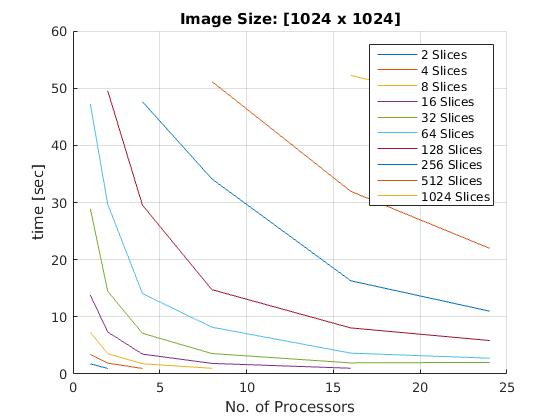
\includegraphics[scale=0.8]{large_one_node_1.jpg}
  \caption{Run time in relation to number of processors for different number of slices. Image size: $[1024 \times 1024]$}
  \label{l_one_n}
\end{figure}

\begin{figure}
  \centering
  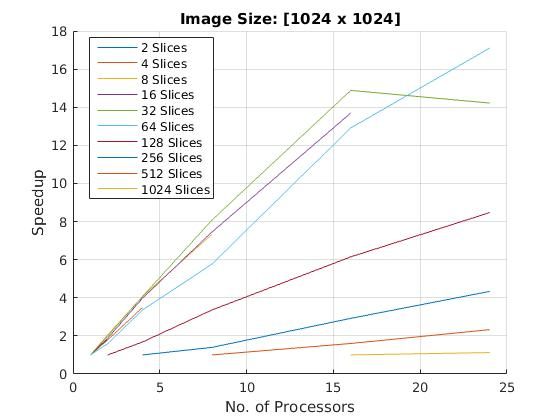
\includegraphics[scale=0.8]{large_one_node_speedup.jpg}
  \caption{Speed-up in relation to number of processors for different number of slices. Image size: $[1024 \times 1024]$}
  \label{l_one_n_speed}
\end{figure}


\begin{figure}
  \centering
  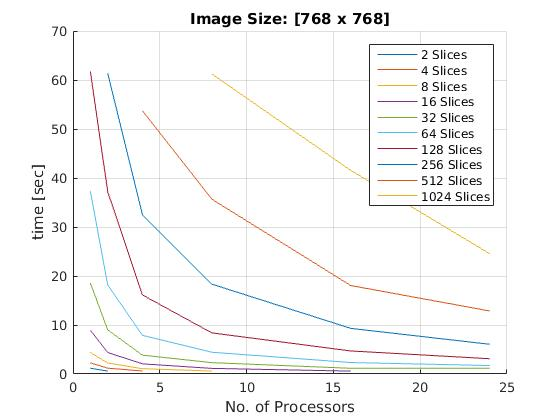
\includegraphics[scale=0.8]{small_one_node_1.jpg}
  \caption{Run time in relation to number of processors for different number of slices. Image size: $[768 \times 768]$}
  \label{s_one_n}
\end{figure}

\begin{figure}
  \centering
  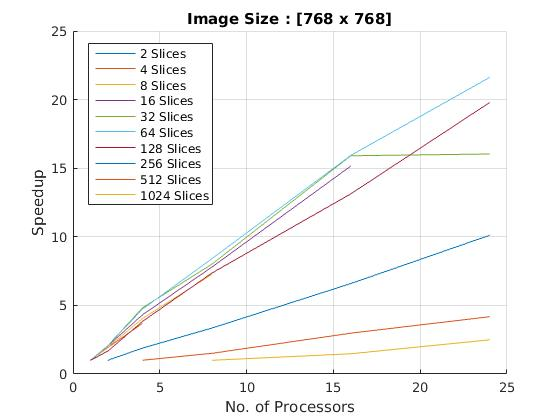
\includegraphics[scale=0.8]{small_one_node_speedup.jpg}
  \caption{Speed-up in relation to number of processors for different number of slices. Image size: $[768 \times 768]$}
  \label{s_one_n_speed}
\end{figure}

Finally we have ran the experiments with 24 processors for both image sizes and increasing number of slices on one and two nodes. In Figure~\ref{nodes} we can see that the run time increases linearly as the work load increases. We can also see that running the experiments on two nodes instead of one has a tiny effect in the run time, which indicates that inter-node communication is insignificant for the nature of this problem.

Table~\ref{table_1} summarizes the speed-ups for varying parameters, the ones that we believe are most indicative and most likely to represent a true experiment.

\begin{figure}
  \centering
  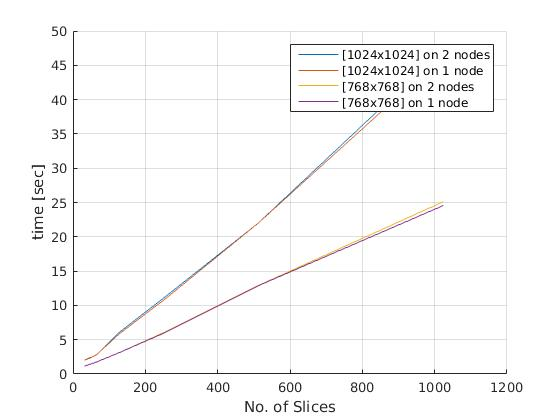
\includegraphics[scale=0.8]{nodes_1.jpg}
  \caption{Run time in relation to number of slices using 24 processors on one and two nodes}
  \label{nodes}
\end{figure}

\begin{table}
\centering
\caption{Speed-ups for different numbers of Processors and Slices}\label{table_1}
    \begin{tabular}{|cc|cc|cc||cc|cc|cc|}
    \hline
    \multicolumn{6}{|c||}{Image Size: $[1024 \times 1024]$} & \multicolumn{6}{|c|}{Image Size: $[768 \times 768]$}\\
    \hline
    \multicolumn{2}{|c|}{64 Slices} & \multicolumn{2}{|c|}{128 Slices} & \multicolumn{2}{|c||}{256 Slices} & \multicolumn{2}{|c|}{64 Slices} & \multicolumn{2}{|c|}{128 Slices} & \multicolumn{2}{|c|}{256 Slices} \\
    \hline

    P  & $S_P$ & P  & $S_P$ & P  & $S_P$ & P  & $S_P$ & P  & $S_P$ & P  & $S_P$ \\ \hline
    1  & 1     & 1  & -     & 1  & -     & 1  & 1     & 1  & 1     & 1  & -     \\
    2  & 1.59  & 2  & 1     & 2  & -     & 2  & 2.05  & 2  & 1.66  & 2  & 1     \\
    4  & 3.35  & 4  & 1.56  & 4  & 1     & 4  & 4.73  & 4  & 3.83  & 4  & 1.89  \\
    8  & 5.77  & 8  & 3.36  & 8  & 1.39  & 8  & 8.4   & 8  & 7.36  & 8  & 3.35  \\
    16 & 12.9  & 16 & 6.15  & 16 & 2.92  & 16 & 15.93 & 16 & 13.13 & 16 & 6.59  \\
    24 & 17.1  & 24 & 8.47  & 24 & 4.33  & 24 & 21.62 & 24 & 19.79 & 24 & 10.11 \\ \hline
    \end{tabular}
\end{table}

\end{document}